%\documentclass[11pt]{article}
\documentclass[twocolumn, prl,showpacs,superscriptaddress]{revtex4-1}   % use preprint or twocolumn
%\usepackage{geometry}                % See geometry.pdf to learn the layout options. There are lots.
%\geometry{letterpaper}                   % ... or a4paper or a5paper or ...
%\geometry{landscape}                % Activate for for rotated page geometry
%\usepackage[parfill]{parskip}    % Activate to begin paragraphs with an empty line rather than an indent
\usepackage{graphicx}
\usepackage{amsmath}
\usepackage{amssymb}
\usepackage{epstopdf}
\usepackage{dcolumn}% Align table columns on decimal point
\usepackage{bm}% bold math

\DeclareGraphicsRule{.tif}{png}{.png}{`convert #1 `dirname #1`/`basename #1 .tif`.png}

\newcommand*{\etal}{\emph{et al.}~}
\newcommand*{\leff}{\lambda_{\textrm{eff}}}
\newcommand*{\lp}{\left(}
\newcommand*{\rp}{\right)}
\newcommand*{\tow}{$\lambda_\textrm{zero}=768.9712(7)_\textrm{stat}(8)_\textrm{sys}$ nm}

\begin{document}

\title{Problem Set 7: Write up}

\author{Charles Griffin}

%%%% Make sure that \maketitle command is after the abstract
\date{\today}
\maketitle
\section{How long does it take before the population stops growing?}
\begin{figure}
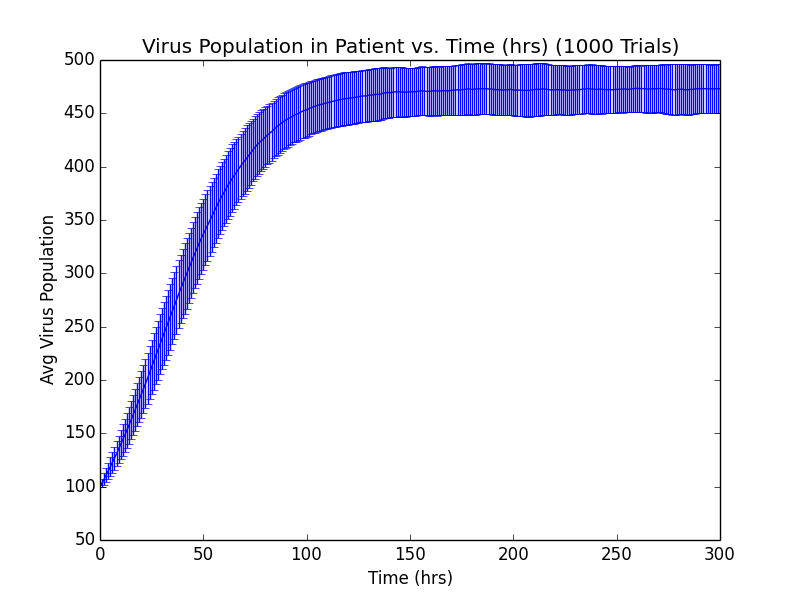
\includegraphics[width=\columnwidth]{./virusPop.png}
\caption{Stochastic model of virus growth without drug treatment.  The population appears to stop increasing (more significantly than the error bars) at around 100 hours.}
\end{figure}
\section{Probability Problems}
\begin{equation}
P(H,H,H) = \left(\frac{1}{2}\right)^3
\end{equation}
\begin{equation}
P(2H,1T) = P(HHT) \times 3C2 = \frac{3}{8}
\end{equation}
\begin{equation}
P(#H>#T) = P(3H)+P(2H,1T) = \frac{1}{8} + \frac{3}{8} = \frac{1}{2}
\end{equation}
\begin{equation}
P(5 of a kind) = \frac{# ways to get 5oK}{# possibilities} = \frac{6}{6^5} = \left(\frac{1}{6}\right)^4
\end{equation}
\end{document}